% Slide: Khung Giao Diện (Wireframe)
\begin{frame}{Khung Giao Diện (Wireframe)}
  \framesubtitle{\color{white!90}\textbf{Hệ thống 32 màn hình chuẩn Mobile-first (iPhone 14 Pro Max)}}

  \begin{columns}[T]
    % Cột trái: Thiết kế & 5 UI States
    \begin{column}{0.50\textwidth}
      {\color{PetcarePrimary}\large \textbf{Quy chuẩn thiết kế \& 5 UI States}}\\[2mm]
      \small
      \begin{itemize}
        \setlength\itemsep{2.2mm}
        \item \textbf{Chuẩn Mobile-first:} Độ phân giải $430 \times 932\text{px}$ tối ưu hóa thao tác một tay trên màn hình lớn.
        \item \textbf{Kiến trúc phẳng:} 4 Phân hệ chính (Trang chủ, Đặt lịch, Tiến độ, Hồ sơ cá nhân).
        \item \textbf{Bao phủ trọn vẹn 5 UI States:}
          \begin{itemize}
            \small \setlength\itemsep{1.2mm}
            \item \textit{Ideal State:} Ma trận giờ còn trống trực quan.
            \item \textit{Loading / Empty:} Skeleton chống giật \& minh họa trống.
            \item \textit{Error / Success:} Cảnh báo đỏ dị ứng \& Mã QR xác nhận.
          \end{itemize}
      \end{itemize}
    \end{column}

    % Cột phải: 3 Màn hình Wireframe
    \begin{column}{0.49\textwidth}
      \centering
      \begin{columns}[c]
        \begin{column}{0.32\textwidth}
          \centering
          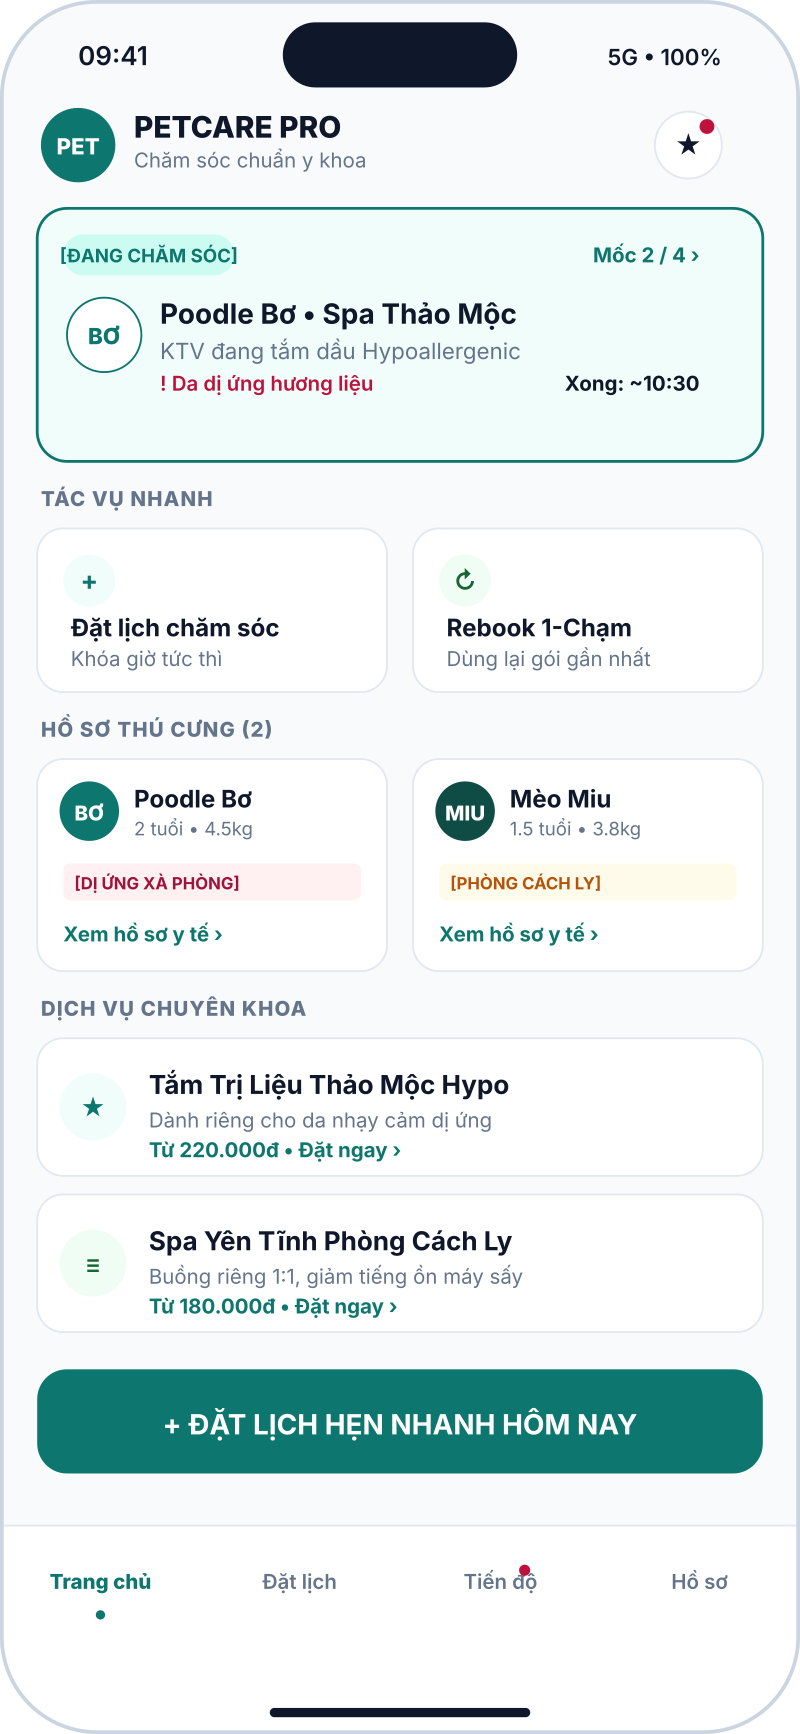
\includegraphics[height=4.6cm, keepaspectratio]{img/wf_01_home.png}\\[1mm]
          {\scriptsize \textbf{Trang chủ}}
        \end{column}
        \begin{column}{0.32\textwidth}
          \centering
          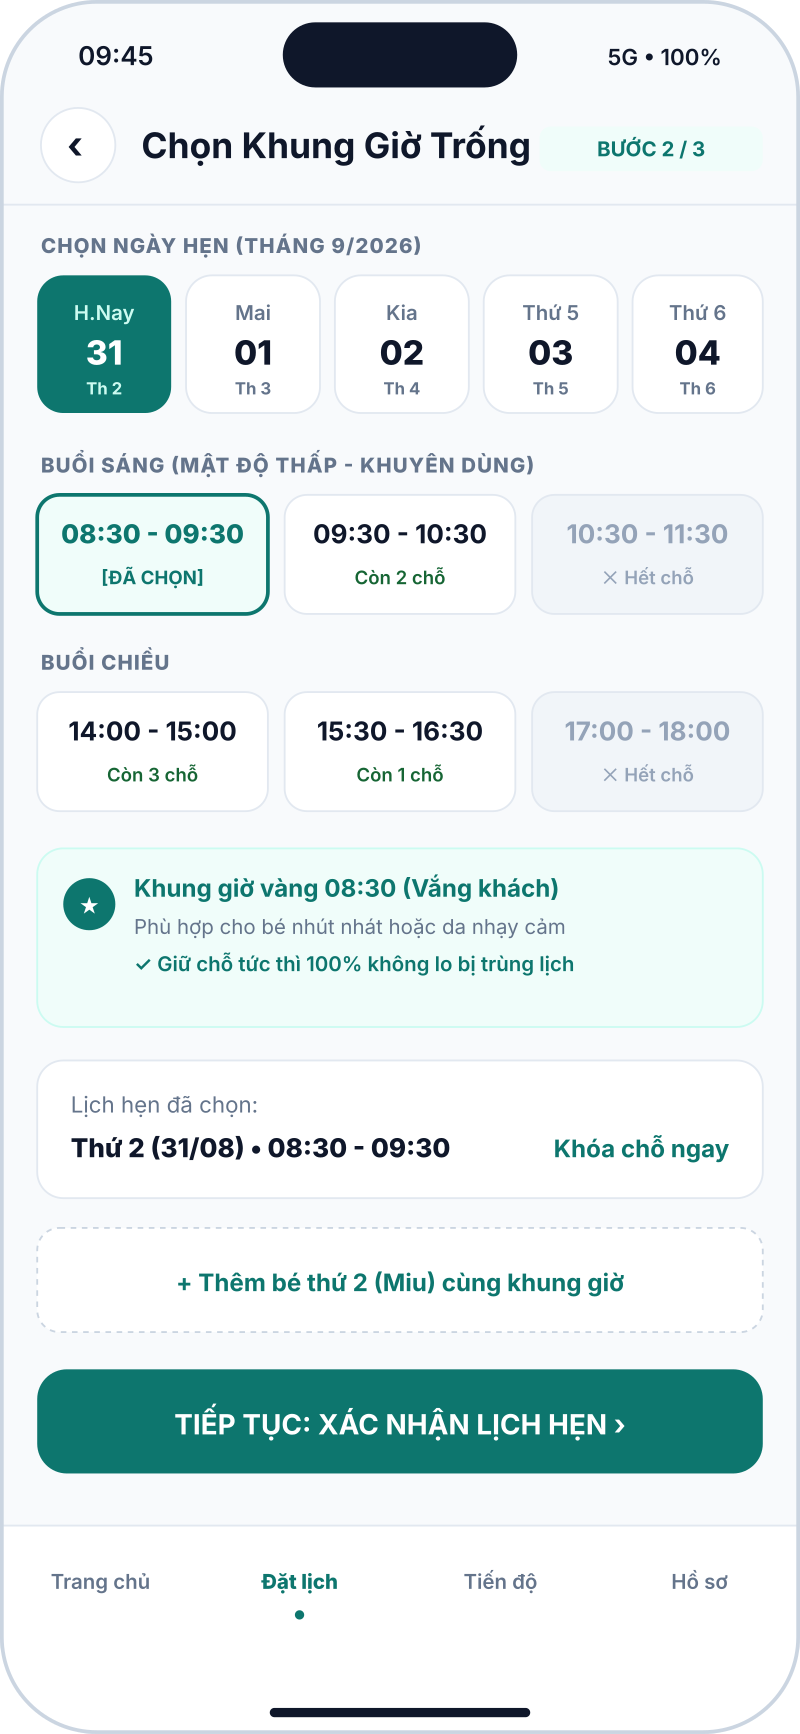
\includegraphics[height=4.6cm, keepaspectratio]{img/wf_05_timeslot.png}\\[1mm]
          {\scriptsize \textbf{Ma trận giờ}}
        \end{column}
        \begin{column}{0.32\textwidth}
          \centering
          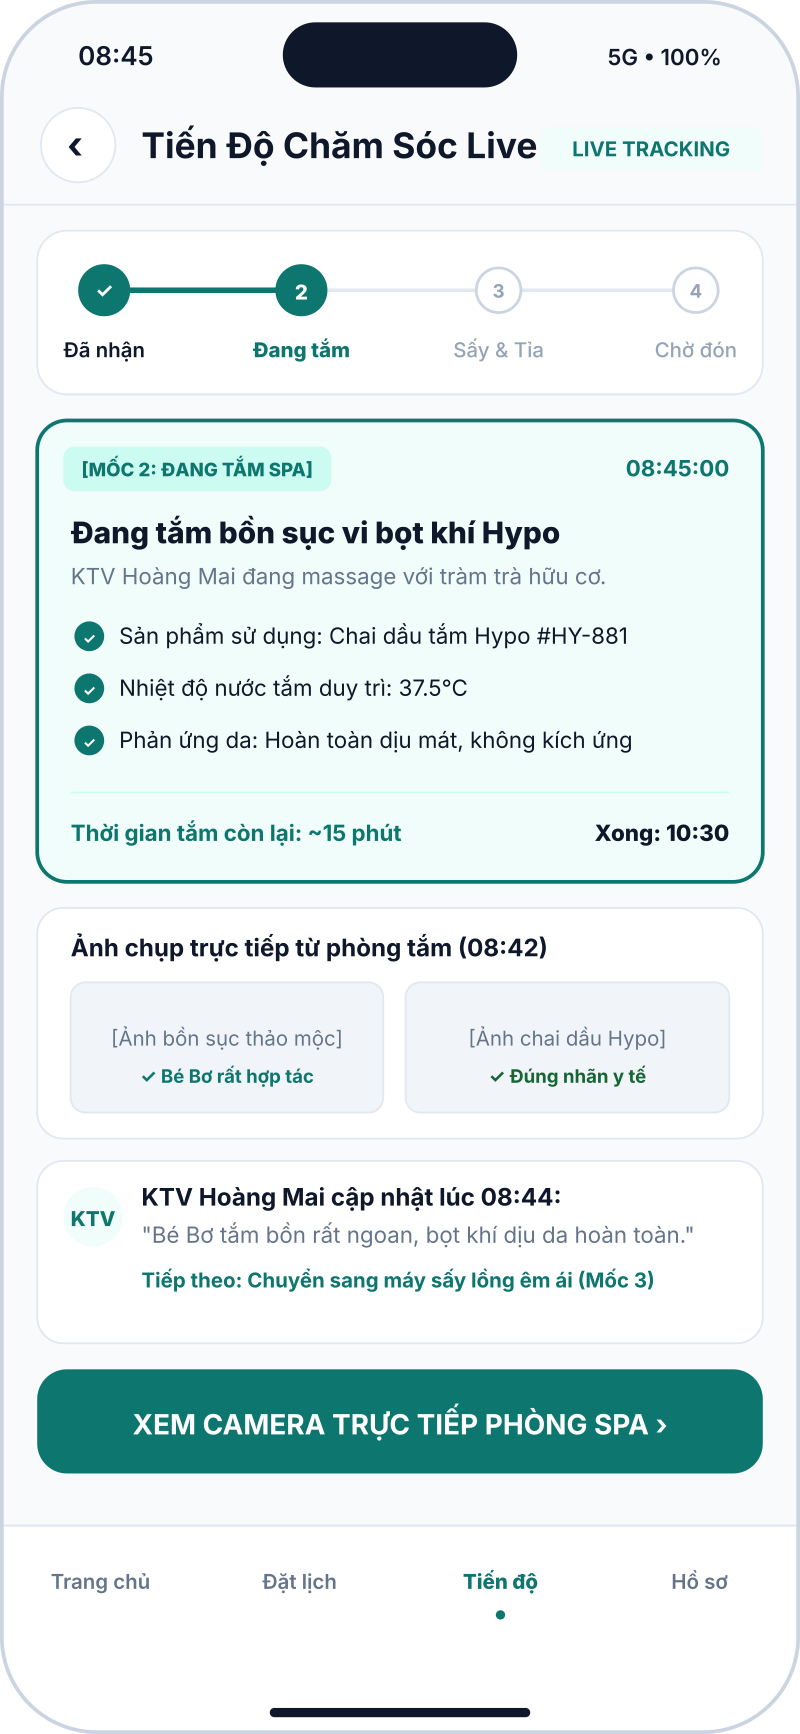
\includegraphics[height=4.6cm, keepaspectratio]{img/wf_15_tracking.png}\\[1mm]
          {\scriptsize \textbf{Tracking}}
        \end{column}
      \end{columns}
    \end{column}
  \end{columns}
\end{frame}
